% Dokumentum konfiguráció
\documentclass[fleqn,12pt]{article}
% --------------------------------------------------
% Dokumentum adatok
% --------------------------------------------------

% Intézmény és kar
\newcommand\INTEZMENY{Budapesti Műszaki és Gazdaságtudományi Egyetem}
\newcommand\KAR{Gépészmérnöki Kar}
\newcommand\LOGO{bme-logo.jpg} % logo fájl neve a figures mappában

% Dokumentum adatok
\newcommand\CIM{Statik 4. Hausaufgabe}
\newcommand\DATUM{2025/26/1}
\newcommand\NEV{Abos Gergő}
\newcommand\NEPTUN{C46M9M}
\newcommand\EMAIL{gergo.abos@gmail.com}
\newcommand\TANTARGY{Statik}
\newcommand\TANTARGYKOD{BMEGEMMBXM1}

% --------------------------------------------------
% Preambulum és egyéni parancsok betöltése
% --------------------------------------------------

\input{../_settings/00_preambulum.tex}
\input{../_settings/01_commands.tex}
\input{../_settings/02_mechTikz.tex}

% ==================================================
% Dokumentum kezdete
% ==================================================
\begin{document}

% Címlap és tartalomjegyzék
% \input{contents/01_title.tex}
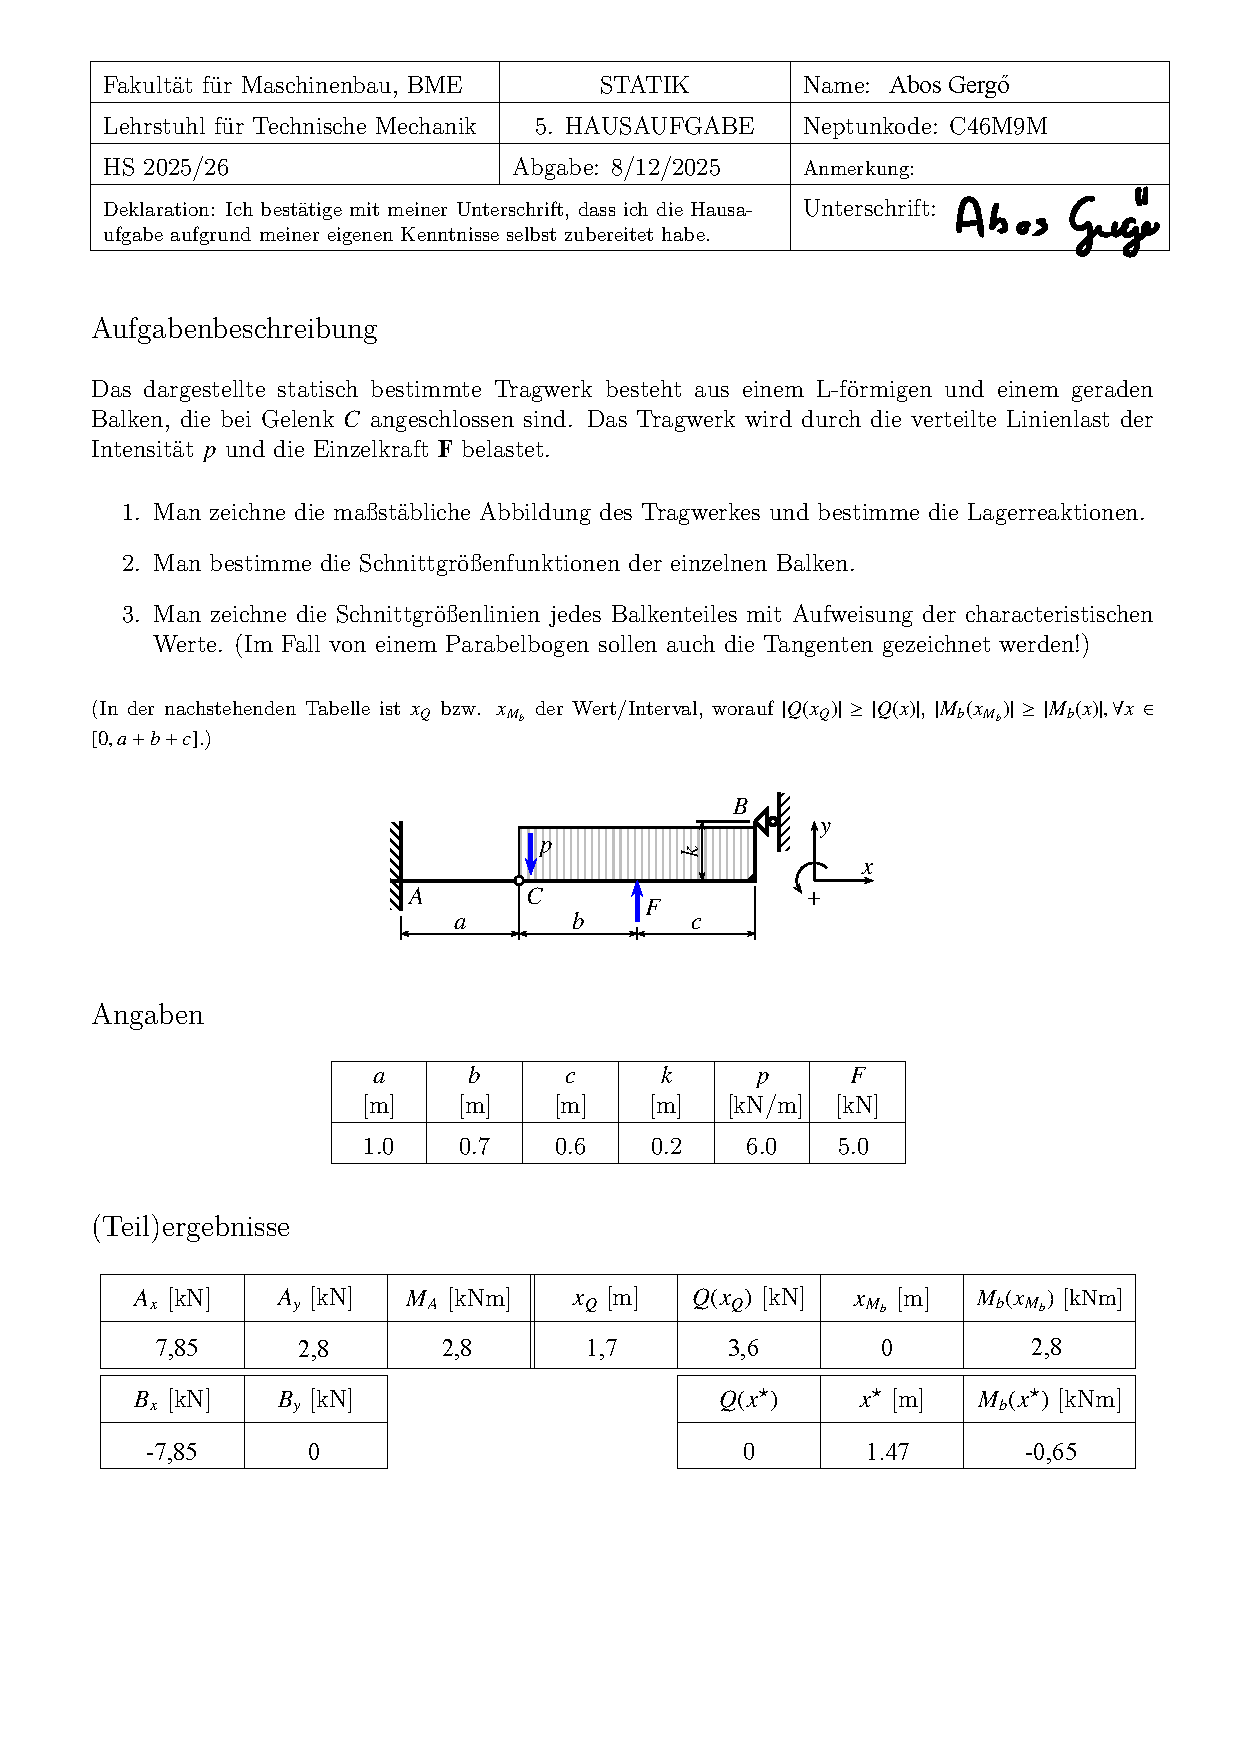
\includepdf[pages=1]{contents/stha5_filled.pdf} % feladatlap beszúrása, ha szükséges
% \input{contents/02_contentpage.tex}
% --------------------------------------------------
% 0. fejezet
% --------------------------------------------------
\section{Maßstäbliche Abbildung, Lagerreaktionen}
\begin{figure}[H]
  \centering
  \begin{tikzpicture}[
      thick, % Default line thickness
      >=Stealth, % Default arrow tip
      force/.style={blue, very thick, ->}, % Style for force arrows
      dimline/.style={thin, <->, >=latex}, % Style for dimension lines
    ]

    % Größen
    \def\masstabm{3cm}
    \def\a{1.0 * \masstabm}
    \def\b{0.7 * \masstabm}
    \def\c{0.6 * \masstabm}
    \def\k{0.2 * \masstabm}

    \def\maßstabN{0.5cm}
    \def\feins{5 * \maßstabN}

    % Koordinaten von Punkte
    \coordinate (A) at (0, 0);
    \coordinate (B) at (\a + \b + \c, \k);
    \coordinate (C) at (\a, 0);
    \coordinate (Corner) at (\a + \b + \c, 0);

    % Beschriftungen von Punkte
    \node[below right]  at (A) {$A$};
    \node[above left] at (B) {$B$};
    \node[below]  at (C) {$C$};

    % Kräfte
    \draw[force] (\a + \b, -\feins) -- (\a + \b, 0) node[below left] {$F$};
    \draw[] (C) -- ($(C) + (0, \k)$) -- (B);
    \fill[pattern=vertical lines] (C) rectangle (B);
    \draw[force, <-] ($(C) + (0.1cm, 0)$) -- ++(0, \k) node[below right] {$p$};

    % Fachwerk Stäber
    \draw[line width=2pt] (A) -- (C) -- (Corner) -- (B);
    \supportroller{B}{90}
    \supportfixed{A}{-90}
    \draw[fill=white, line width=2pt] (C) circle (0.08cm);
  \end{tikzpicture}
  \caption{Maßstäbliche Abbildung des Tragwerkes}
\end{figure}

Um den Lagerreaktionen zu bestimmen zeichne ich für jeden Balken ein Freikörperbild. Das verteilte Kraft $p$ wurde durch ein Einzelkraft $F_p$ ersetzt:
\begin{align*}
  F_p = p \cdot (b + c) = 6 \cdot 1.3 = 7,8\text{ kN} & &x_p = a + \frac{b + c}{2} = 1.65\text{ m}
\end{align*}

\begin{figure}[H]
  \centering
  \begin{minipage}[b]{0.48\textwidth}
    \centering
    \begin{tikzpicture}[
        thick, % Default line thickness
        >=Stealth, % Default arrow tip
        force/.style={blue, very thick, ->}, % Style for force arrows
        dimline/.style={thin, <->, >=latex}, % Style for dimension lines
      ]

      % Größen
      \def\masstabm{3cm}
      \def\a{1.0 * \masstabm}
      \def\b{0.7 * \masstabm}
      \def\c{0.6 * \masstabm}
      \def\k{0.2 * \masstabm}

      \def\maßstabN{0.5cm}

      % Koordinaten von Punkte
      \coordinate (A) at (0, 0);
      \coordinate (B) at (\a + \b + \c, \k);
      \coordinate (C) at (\a, 0);
      \coordinate (Corner) at (\a + \b + \c, 0);

      % Beschriftungen von Punkte
      \node[below right]  at (A) {$A$};
      \node[below left]  at (C) {$C$};

      \draw[force] (A) -- ($(A) + (0, \maßstabN * 2)$) node[right] {$A_Y$};
      \draw[force] ($(A) + (-\maßstabN * 2, 0)$) -- (A) node[below left] {$A_X$};
      \draw[force] ($(A) + (45:0.5cm)$) arc[start angle = 45, end angle=150, radius=0.5cm] node[above left] {$M_A$};

      \draw[force] (C) -- ($(C) + (0, \maßstabN * 2)$) node[right] {$C_Y$};
      \draw[force] (C) -- ($(C) + (\maßstabN * 2, 0)$) node[below left] {$C_X$};
      % Fachwerk Stäber
      \draw[line width=2pt] (A) -- (C);
    \end{tikzpicture}
    \caption{Freikörperbild zum Balken 1}
  \end{minipage}
  \begin{minipage}[b]{0.48\textwidth}
    \centering
    \begin{tikzpicture}[
        thick, % Default line thickness
        >=Stealth, % Default arrow tip
        force/.style={blue, very thick, ->}, % Style for force arrows
        dimline/.style={thin, <->, >=latex}, % Style for dimension lines
      ]

      % Größen
      \def\masstabm{3cm}
      \def\a{1.0 * \masstabm}
      \def\b{0.7 * \masstabm}
      \def\c{0.6 * \masstabm}
      \def\k{0.2 * \masstabm}

      \def\maßstabN{0.25cm}
      \def\feins{5 * \maßstabN}
      \def\fp{7.8 * \maßstabN}

      % Koordinaten von Punkte
      \coordinate (A) at (0, 0);
      \coordinate (B) at (\a + \b + \c, \k);
      \coordinate (C) at (\a, 0);
      \coordinate (Corner) at (\a + \b + \c, 0);

      % Beschriftungen von Punkte
      \node[above left] at (B) {$B$};
      \node[above]  at (C) {$C$};

      % Kräfte
      \draw[force] (\a + \b, -\feins) -- (\a + \b, 0) node[below left] {$F$};
      \draw[force, <-] ($(C)!0.5!(Corner)$) -- ++(0, \fp) node[below left] {$F_p$};

      \draw[force] (C) -- ($(C) + (0, -\maßstabN * 4)$) node[right] {$C_Y$};
      \draw[force] (C) -- ($(C) + (-\maßstabN * 4, 0)$) node[below] {$C_X$};

      \draw[force] (B) -- ($(B) + (\maßstabN * 4, 0)$) node[below left] {$B_X$};
      % Fachwerk Stäber
      \draw[line width=2pt] (C) -- (Corner) -- (B);
    \end{tikzpicture}
    \caption{Freikörperbild zum Balken 2}
  \end{minipage}
\end{figure}
Für beide Balken gelten 3 Gleichgewichtsgleichungen:
\begin{align*}
  &\sum F_X = A_X + C_X = 0 & &\sum F_X = B_X - C_X = 0 \\
  &\sum F_Y = A_Y + C_Y = 0 & &\sum F_Y = F - F_p - C_Y = 0 \\
  &\sum M_C = A_M - A_Y \cdot a = 0 & &\sum M_C = F \cdot b - F_p \cdot \frac{b + c}{2} - B_X \cdot k = 0
\end{align*}
Davon bekommt:
\begin{center}
  \boxed{
    \begin{aligned}
      &A_X = 7,85\text{ kN} & &C_X = -7,8\text{ kN}\\
      &A_Y = 2,8\text{ kN} & &C_Y = -2,8\text{ kN} \\
      &M_A = 2,8\text{ kNm}& &B_X = -7,85\text{ kN}\\
    \end{aligned}
  }
\end{center}

\section{Schnittgrößenfunktionen der Balken}
\subsection{Definition der Koordinatensystem}
Das Tragwerk will immer im Laufpunkt $x$ in zwei Teile geschneiden werden:
\begin{figure}[H]
  \centering
  \begin{tikzpicture}[
      thick, % Default line thickness
      >=Stealth, % Default arrow tip
      force/.style={blue, very thick, ->}, % Style for force arrows
      dimline/.style={thin, <->, >=latex}, % Style for dimension lines
    ]

    % Größen
    \def\masstabm{3cm}
    \def\a{1.0 * \masstabm}
    \def\b{0.7 * \masstabm}
    \def\c{0.6 * \masstabm}
    \def\k{0.2 * \masstabm}

    \def\massstabN{0.5cm}
    \def\feins{5 * \massstabN}

    % Koordinaten von Punkte
    \coordinate (A) at (0, 0);
    \coordinate (B) at (\a + \b + \c, \k);
    \coordinate (C) at (\a, 0);
    \coordinate (Corner) at (\a + \b + \c, 0);

    % Beschriftungen von Punkte
    \node[above]  at (A) {$A$};
    \node[left] at (B) {$B$};
    \node[above]  at (C) {$C$};

    % Fachwerk Stäber
    \draw[line width=2pt] (A) -- (C) -- (Corner) -- (B);
    \draw[line width=2pt, dotted, ->, red] ($(A) - (0, 0.2cm)$) -- ($(Corner) - (-0.2cm, 0.2cm)$) -- ($(B) + (0.2cm, 0)$) node[below right] {$x$};
  \end{tikzpicture}
  \caption{Definition der Koordinatensystem}
  \label{fig:Koordinatensystem}
\end{figure}
Aus dieser Definition kommt: $x \in [0, a + b + c + k]$.

Die rote Linie auf \figref{fig:Koordinatensystem} definiert die Unterseite der Stäber auch.
\subsection{Vorzeichenkonvention}
Nach der Konvention werden die Folgende Vorzeichenkonventionen benutzt:
\begin{itemize}
  \item Normalkräfte $N(x)$: Poisitive Werte representieren Zug, negative Werte representieren Druck
  \item Querkräfte $Q(x)$: Positive Werte verursachecn eine Drehung im Uhrzeigersinn.
  \item Biegemomente $M_b(x)$: Bei positive Werte wird die Obere Seite des Balkens gezogen, die untere Seite gedruckt.
\end{itemize}
\subsection{Schnittbereiche bestimmen}
Das Tragwerk muss auf 4 Teile geteilt werden. Für jeden Teil müssen verschiede Schnittgrößenfunktionen aufgeschrieben werden. Die 3 Teilpunkte sind:
\begin{enumerate}
  \item Punkt C, da das verteilten Kraft dort beginnt.
  \item Angriffspunkt von F
  \item Eckpunkt der Balken, da dort die Normalkräfte und Querkräfte getauscht sind. (Das Balken biegt $90^\circ$) Das verteilte Kraft beendet sich dort auch.
\end{enumerate}
\begin{figure}[H]
  \centering
  \begin{tikzpicture}[
      thick,
      >=Stealth,
      force/.style={blue, very thick, ->},
      dimline/.style={thin, <->, >=latex},
      schnitt/.style={red, dashed, very thick}
    ]

    % Größen
    \def\masstabm{3cm}
    \def\a{1.0 * \masstabm}
    \def\b{0.7 * \masstabm}
    \def\c{0.6 * \masstabm}
    \def\k{0.2 * \masstabm}

    \def\maßstabN{0.5cm}
    \def\feins{5 * \maßstabN}

    % Koordinaten von Punkte
    \coordinate (A) at (0, 0);
    \coordinate (B) at (\a + \b + \c, \k);
    \coordinate (C) at (\a, 0);
    \coordinate (Corner) at (\a + \b + \c, 0);

    % Beschriftungen von Punkte
    \node[below right]  at (A) {$A$};
    \node[above left] at (B) {$B$};
    \node[below left]  at (C) {$C$};

    % Kräfte
    \draw[force] (\a + \b, -\feins) -- (\a + \b, 0) node[below left] {$F$};
    \draw[] (C) -- ($(C) + (0, \k)$) -- (B);
    \fill[pattern=vertical lines] (C) rectangle (B);
    \draw[force, <-] ($(C) + (0.1cm, 0)$) -- ++(0, \k) node[below right] {$p$};
    \draw[force] (B) -- ($(B) + (\maßstabN * 2, 0)$) node[below left] {$B_X$};
    \draw[force] (A) -- ($(A) + (0, \maßstabN * 2)$) node[right] {$A_Y$};
    \draw[force] ($(A) + (-\maßstabN * 2, 0)$) -- (A) node[below left] {$A_X$};
    \draw[force] ($(A) + (45:0.5cm)$) arc[start angle = 45, end angle=150, radius=0.5cm] node[above left] {$M_A$};

    % Tragwerk
    \draw[line width=2pt] (A) -- (C) -- (Corner) -- (B);
    \draw[fill=white, line width=2pt] (C) circle (0.08cm);

    % -----------------------------------------------------
    % Schnittlinien
    % -----------------------------------------------------

    % S1: bei C
    \draw[schnitt] ($(C)+(0,-0.6)$) -- ($(C)+(0,0.6)$);
    \node[red] at ($(C)+(0.3,-0.4)$) {$S_1$};

    % S2: Angriffspunkt F, also bei (a+b, 0)
    \coordinate (Fpoint) at (\a + \b, 0);
    \draw[schnitt] ($(Fpoint)+(0,-0.6)$) -- ($(Fpoint)+(0,0.6)$);
    \node[red] at ($(Fpoint)+(0.3,-0.4)$) {$S_2$};

    % S3: Eckpunkt des Balkens (Corner)
    \draw[schnitt] ($(Corner)+(0.6,-0.6)$) -- ($(Corner)+(-0.6,0.6)$);
    \node[red] at ($(Corner)+(0,-0.4)$) {$S_3$};

  \end{tikzpicture}
  \caption{Die vier Schnittbereiche}
\end{figure}
\subsection{Schnittgrößenfunktionen bestimmen}
Nach einem Schnitt im Punkt $x$ wird die rechte Seite von $x$ ($[x, a + b + c + k]$) verlassen werden.
In der Funktionen werden die bleibende Kräfte und Momente (die auf den Intervall $[0, x]$ liegen) eingeschrieben.
\begin{align*}
  x &\in~\rbrack 0, a \lbrack & x &\in~\rbrack a, a + b \lbrack\\
  N(x) &= -A_X = -7,85 & N(x) &= -A_X = -7,85 \\
  Q(x) &= A_Y = 2,8kN & Q(x) &= A_Y - p \cdot (x - a) = 8,8 - 6x\\
  M_b(x) &= M_A - A_Y \cdot x = 2,8 - 2,8x & M_b(x) &= M_A - A_Y \cdot x + p \cdot \frac{(x - a)^2}{2} = \\
  & & &= 3x^2 - 8,8x + 5,8 \\
\end{align*}
\begin{align*}
  x &\in~\rbrack a + b, a + b + c \lbrack\\
  N(x) &= -A_X = -7,85 \\
  Q(x) &= A_Y - p \cdot (x - a) + F = 13,8 - 6x\\
  M_b(x) &= M_A - A_Y \cdot x + p \cdot \frac{(x - a)^2}{2} - F \cdot (x - a + b) = 3x^2 - 7,8x + 8,3
\end{align*}
Bei dem letzten Teil ($x \in~\rbrack a + b + c, a + b + c + k \lbrack$) liegt das Stab senkrecht auf der vorherigen Stäber. Deswegen werden bisherige Normalkräfte als Querkräfte angenommen, bzw. Querkräfte als Normalkräfte. Es ist auch einfacher, die andere Seite des Tragwerkes zu verlassen, so ist es nötig nur mit einer Kraft zu rechnen.
\begin{align*}
  x &\in~\rbrack a + b + c, a + b + c + k \lbrack\\
  N(x) &= 0 \\
  Q(x) &= B_X = 7,85 \\
  M_b(x) &= (a + b + c + k - x) \cdot B_X = -19,625 + 7,85x
\end{align*}

\section{Schnittgrößenlinien}
In folgendem werden die Schnittgrößenfunktionen dargestellt. Die vertikale Achse wird die x-Koordinate immer. Die Funktions, und alle berühmte Funktionswerte sind mit blau dargestellt. Bei ener Parabel sind die Extremwerte (Minimum, Maximum), und die Schnittpunkt der Tangenten im Anfang- und Endpunkt auch gezeichnet.
Die x-Koordinaten der Schnittpunkte sind nicht dargestellt, weil die sind immer die Mittelpunkt der zwei Punkte wo die Tangenten gezeicht sind. Das kommt aus der Definition einer Parabel.
\begin{figure} [H]
  \centering
  \begin{tikzpicture}
    \def\xscale{5}
    \def\yscale{0.25}

    \def\a{1   * \xscale}
    \def\b{0.7 * \xscale}
    \def\c{0.6 * \xscale}
    \def\k{0.2 * \xscale}

    \def\N{-7.85}
    \def\Ay{2.8}
    \def\p{6}
    \def\F{5}
    \def\Bx{-7.85}
    \def\Ma{2.8}

    %%%%%%%%%%%%%%%%%%%%%%%%%%%%%%%%%%%%%%%%%%%%%%%%%%%%%%%
    %  Vertical guider lines
    %%%%%%%%%%%%%%%%%%%%%%%%%%%%%%%%%%%%%%%%%%%%%%%%%%%%%%%
    \foreach \X in {0, \a, \a+\b, \a+\b+\c, \a+\b+\c+\k} {
      \draw[dashed, gray] (\X, 14 * \yscale) -- (\X, -55 * \yscale);
    }

    \begin{scope}[yshift=14cm*\yscale, force/.style={blue, very thick, ->}, >=Stealth]
      \def\maßstabN{0.5cm}
      \def\feins{5 * \maßstabN}

      % Koordinaten von Punkte
      \coordinate (A) at (0, 0);
      \coordinate (B) at (\a + \b + \c, \k);
      \coordinate (C) at (\a, 0);
      \coordinate (Corner) at (\a + \b + \c, 0);

      % Beschriftungen von Punkte
      \node[below right]  at (A) {$A$};
      \node[above left] at (B) {$B$};
      \node[below]  at (C) {$C$};

      % Kräfte
      \draw[force] (\a + \b, -\feins) -- (\a + \b, 0) node[below left] {$F$};
      \draw[blue] (C) -- ($(C) + (0, \k)$) -- (B);
      \fill[pattern=vertical lines, pattern color = blue] (C) rectangle (B);
      \draw[force, <-] ($(C) + (0.1cm, 0)$) -- ++(0, \k) node[below right] {$p$};

      % Fachwerk Stäber
      \draw[dashed, gray] (B) arc[start angle=90, end angle=0, radius=\k];
      \draw[line width=2pt] (A) -- (C) -- (Corner) -- (B);
      \draw[force] (A) -- ($(A) + (0, \maßstabN * 2)$) node[right] {$A_Y$};
      \draw[force] ($(A) + (-\maßstabN * 2, 0)$) -- (A) node[below left] {$A_X$};
      \draw[force] ($(A) + (45:0.5cm)$) arc[start angle = 45, end angle=150, radius=0.5cm] node[above left] {$M_A$};
      \draw[fill=white, line width=2pt] (C) circle (0.08cm);
      \draw[force] (B) -- ($(B) + (\maßstabN * 2, 0)$) node[below left] {$B_X$};
    \end{scope}

    %%%%%%%%%%%%%%%%%%%%%%%%%%%%%%%%%%%%%%%%%%%%%%%%%%%%%%%
    % 1st graph:  N(x)
    %%%%%%%%%%%%%%%%%%%%%%%%%%%%%%%%%%%%%%%%%%%%%%%%%%%%%%%
    % Axes
    \draw[->] (0,0) -- (2.8 * \xscale,0) node[below] {$x$};
    \draw[->] (0,-8 * \yscale) -- (0, 2 * \yscale) node[left] {$N(x)$};
    \draw[->] (0,-8 * \yscale) -- (0, 2 * \yscale) node[right] {$[kN]$};

    % Step shape for N
    \draw[blue, line width=1.5pt]
    (0, \N * \yscale) --
    (\a+\b+\c, \N * \yscale) --
    (\a+\b+\c, 0) --
    (\a+\b+\c+\k, 0);

    % Shaded area
    \fill[pattern=vertical lines, pattern color=blue]
    (0,0) -- plot[domain=0:\a+\b+\c] (\x, {\N * \yscale})
    -- (\a+\b+\c,0);

    % Labels
    \node[left, blue] at (0, \N * \yscale) {$-7.85$};
    \node[left] at (0, 0) {$0$};

    %%%%%%%%%%%%%%%%%%%%%%%%%%%%%%%%%%%%%%%%%%%%%%%%%%%%%%%
    % 2nd graph: Q(x) with jumps
    %%%%%%%%%%%%%%%%%%%%%%%%%%%%%%%%%%%%%%%%%%%%%%%%%%%%%%%
    \begin{scope}[yshift=-19cm*\yscale]
      \def\yscale{0.5}

      % Axes
      \draw[->] (0,0) -- (2.8 * \xscale,0) node[below] {$x$};
      \draw[->] (0,-7.85 * \yscale) -- (0,4 * \yscale) node[left] {$Q(x)$};
      \draw[->] (0,-7.85 * \yscale) -- (0,4 * \yscale) node[right] {$[kN]$};

      % First segment
      \draw[blue, line width=1.5pt, domain=0:\a]
      plot (\x, {\Ay * \yscale});
      \fill[pattern=vertical lines, pattern color=blue]
      (0,0) -- plot[domain=0:\a] (\x, {\Ay * \yscale}) -- (\a,0);

      % Second segment
      \draw[blue, line width=1.5pt, domain=\a:\a+\b]
      plot (\x, {(\Ay + \p - \p * \x / \xscale) * \yscale});
      \fill[pattern=vertical lines, pattern color=blue]
      (\a,0) --
      plot[domain=\a:\a+\b] (\x, {(\Ay + \p - \p * \x / \xscale) * \yscale})
      -- (\a+\b,0);

      % Third segment
      \draw[blue, line width=1.5pt, domain=\a+\b:\a+\b+\c]
      plot (\x, {(\Ay + \p + \F - \p * \x / \xscale) * \yscale});
      \fill[pattern=vertical lines, pattern color=blue]
      (\a+\b,0) --
      plot[domain=\a+\b:\a+\b+\c]
      (\x, {(\Ay + \p + \F - \p * \x / \xscale) * \yscale})
      -- (\a+\b+\c,0);

      % Final constant segment
      \draw[blue, line width=1.5pt, domain=\a+\b+\c:\a+\b+\c+\k]
      plot (\x, {\Bx * \yscale});
      \fill[pattern=vertical lines, pattern color=blue]
      (\a+\b+\c,0) --
      plot[domain=\a+\b+\c:\a+\b+\c+\k] (\x, {\Bx * \yscale})
      -- (\a+\b+\c+\k,0);

      % Vertical jumps
      \draw[blue, line width=1.5pt] (\a+\b, 3.6 * \yscale) -- (\a+\b, -1.4 * \yscale);
      \draw[blue, line width=1.5pt] (\a+\b+\c, 0) -- (\a+\b+\c, -7.85 * \yscale);
      \draw[blue, line width=1.5pt] (\a+\b+\c+\k, 0) -- (\a+\b+\c+\k, -7.85 * \yscale);

      % Labels
      \node[left, blue] at (0,\Ay * \yscale) {$\Ay$};
      \node[left] at (0,0) {$0$};
      \node[blue, right] at (\a+\b, -1.4 * \yscale) {$-1.4$};
      \node[blue, left] at (\a+\b, 3.6 * \yscale) {$3.6$};
      \node[blue, left] at (\a+\b+\c, -7.85 * \yscale) {$-7.85$};
      \node[above] at (8.8 * \xscale / 6, 0) {$1.47$};

    \end{scope}

    %%%%%%%%%%%%%%%%%%%%%%%%%%%%%%%%%%%%%%%%%%%%%%%%%%%%%%%
    % 3rd graph: the smoothed Q(x)
    %%%%%%%%%%%%%%%%%%%%%%%%%%%%%%%%%%%%%%%%%%%%%%%%%%%%%%%
    \begin{scope}[yshift=-50cm*\yscale]
      \def\yscale{0.75}
      % Axes
      \draw[->] (0,0) -- (2.8 * \xscale,0) node[below] {$x$};
      \draw[->] (0,-2 * \yscale) -- (0,4 * \yscale) node[left] {$M_b(x)$};
      \draw[->] (0,-2 * \yscale) -- (0,4 * \yscale) node[right] {$[kNm]$};

      % Smooth First segment
      \draw[blue, line width=1.5pt, domain=0:\a]
      plot (\x, {( \Ma - \x / \xscale * \Ay ) * \yscale});
      \fill[pattern=vertical lines, pattern color=blue]
      (0,0) --
      plot[domain=0:\a] (\x,{(\Ma - \x / \xscale * \Ay) * \yscale})
      -- (\a,0);

      % Smooth Second
      \draw[blue, line width=1.5pt, domain=\a:\a+\b]
      plot (\x, {( \Ma - \x/\xscale * \Ay + \p*((\x-\a)/\xscale)^2/2 ) * \yscale});
      \fill[pattern=vertical lines, pattern color=blue]
      (\a,0) --
      plot[domain=\a:\a+\b]
      (\x,{(\Ma - \x/\xscale * \Ay + \p*((\x-\a)/\xscale)^2/2 ) * \yscale})
      -- (\a+\b,0);

      % Smooth Third
      \draw[blue, line width=1.5pt, domain=\a+\b:\a+\b+\c]
      plot (\x,{(\Ma - \x/\xscale * \Ay + \p*((\x-\a)/\xscale)^2/2 - \F*(\x-\a-\b)/\xscale ) * \yscale});
      \fill[pattern=vertical lines, pattern color=blue]
      (\a+\b,0) --
      plot[domain=\a+\b:\a+\b+\c]
      (\x,{(\Ma - \x/\xscale * \Ay + \p*((\x-\a)/\xscale)^2/2 - \F*(\x-\a-\b)/\xscale ) * \yscale})
      -- (\a+\b+\c,0);

      \draw[blue, dashed, domain=\a:\a+\b/2] plot (\x, {(2.8 - 2.8 * \x / \xscale) * \yscale});
      \draw[blue, dashed, domain=\a+\b/2:\a+\b] plot (\x, {(-2.87 + 1.4 * \x / \xscale) * \yscale});
      \fill[blue] (\a+\b/2, -0.98cm * \yscale) circle (0.05cm);

      \draw[blue, dashed, domain=\a+\b:\a+\b+\c/2] plot (\x, {(5.63 - 3.6 * \x / \xscale) * \yscale});
      \draw[blue, dashed, domain=\a+\b+\c/2:\a+\b+\c] plot (\x, {(-1.57) * \yscale});
      \fill[blue] (\a+\b+\c/2, -1.57cm * \yscale) circle (0.05cm);

      % Final smooth segment
      \draw[blue, line width=1.5pt, domain=\a+\b+\c:\a+\b+\c+\k]
      plot (\x,{(\a+\b+\c+\k-\x)/\xscale * \Bx * \yscale});
      \fill[pattern=vertical lines, pattern color=blue]
      (\a+\b+\c,0) --
      plot[domain=\a+\b+\c:\a+\b+\c+\k]
      (\x,{(\a+\b+\c+\k-\x)/\xscale * \Bx * \yscale})
      -- (\a+\b+\c+\k,0);

      % Labels
      \node[left, blue] at (0,\Ay * \yscale) {$\Ay$};
      \node[below, blue] at (\a+\b/2, -0.98 * \yscale) {$-0,98$};
      \draw[blue, dashed] (1.47*\xscale, -0.65*\yscale) -- (1*\xscale, -0.65*\yscale);
      \node[left, blue] at (1*\xscale, -0.65*\yscale) {$-0,65$};
      \node[below, blue, xshift=-5] at (\a+\b, -0.49 * \yscale) {$-0,49$};
      \node[below, blue] at (\a+\b+\c, -1.57 * \yscale) {$-1,57$};
      \node[below, blue] at (\a+\b+\c/2, -1.57 * \yscale) {$-1,57$};
      \node[left] at (0,0) {$0$};

    \end{scope}

  \end{tikzpicture}
\end{figure}
\subsection{Überprüfung mit Ablesung}
Es gibt einige zusammenhänge zwischen die Funktionen, die kann man kontrollieren. $M_b(x)$ ist die negative Ableitung von $Q(x)$. Das heißt, dass wo $Q(x) = 0$ ist, dort sollen die Parabelfunktionen ein Extremwert haben. An der ende des Stabes (Punkt B) gibt kein konzentriertes Kräftepaar (Moment). Deswegen soll der Biegemoment dort 0 sein. Das selbe ist wahr für Normalkräfte. Die Funktionsgraphe zeigen diese Eigenschaften.
Im Punkt C gibt es ein Gelenk. In diesem Punkt soll $M_b(a) = 0$ sein, weil das Gelenk das Freiheit nur translatorisch begrenzt.

\section{Überprüfung mit Computer-Rechnung}
Das Tragwerk wurde auf die Webseite \href{https://run.edubeam.app/?model=eyJuIjpbWyIxIixbMCwwLDBdLFswLDQsMl0sbnVsbF0sWyIyIixbMSwwLDBdLFtdLG51bGxdLFsiMyIsWzIuMywwLDBdLFtdLG51bGxdLFsiNCIsWzIuMywwLC0wLjJdLFswXSxudWxsXV0sImUiOltbIjEiLFsiMSIsIjIiXSwiMSIsIjEiLFtmYWxzZSx0cnVlXV0sWyIyIixbIjIiLCIzIl0sIjEiLCIxIixbZmFsc2UsZmFsc2VdXSxbIjMiLFsiMyIsIjQiXSwiMSIsIjEiLFtmYWxzZSxmYWxzZV1dXSwibSI6W1siMSIsNDAwMCwyMTAwMDAwMDAwMDAsODc1MDAwMDAwMDAsMC4wMDAwMTJdXSwiY3MiOltbIjEiLDEsMC4wMDAwODM1NiwxLDFlKzMyXV0sImVsIjpbWyIyIixbMCw2MDAwXSx0cnVlXV0sImVjbCI6W1siMiIsWzAsLTUwMDAsMCwwLjddLHRydWVdXSwiZCI6W119#}{Edubeam} modelliert.
\begin{figure}[H]
  \centering
  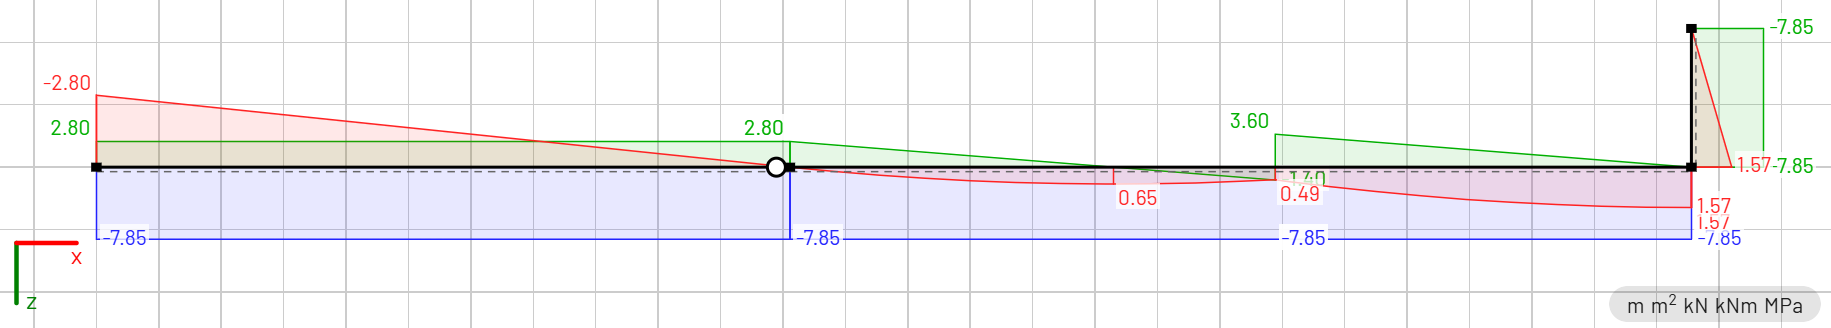
\includegraphics[width=\textwidth]{contents/edubeam.png}
  \caption{Ergebnis der Analyse}
  \label{fig:edubeam}
\end{figure}
Auf \figref{fig:edubeam} kann $N(x)$ mit blau, $Q(x)$ mit grün, und $M_b(x)$ mit rot gezeichet sehen.
Die Lösüngen von $N(x)$ und $Q(x)$ übereinstimmen. $M_b(x)$ ist gegenseitig gleich groß, als die vorhere Lösüng. Diese Unterschied kommt aus der Ursache, dass die Webseite benutzt die gegenseitige Konvention für Biegemoment. Die vorher gegebene Lösungen sind also richtig.
\end{document}
